\section{Evaluation}

\comment{

Giza provides fault tolerance through erasure coding across wide area networks while providing strong consistency for its read and write operations. There is currently no system that is specifically designed to serve as an alternative to Giza. As such, we benchmark Giza’s performance against Cassandra and CockroachDB to illustrate the following points:

- In the common case, Giza’s Fast Paxos implementation of the metadata phase allows for lower latency writes for Giza when compared to Cassandra.

- While one could implement Giza’s metadata phase and data phase as a single distributed transaction, we illustrate through CockroachDB that doing so will degrade performance significantly.

In addition, we provide evaluation results for encoding scheme ranging from 2-1 in 3 data centers to 18-4 in 22 data centers to illustrate the flexibility of Giza as a front end.

}

For evaluation, we deploy Giza on top of the Microsoft Azure platform across 11 data centers (7 in North America, 2 in Europe and 2 in Asia). For each data center, we deploy virtual machines as Giza nodes. As describe in Section~\ref{sec:design}, all the Giza nodes are stateless. Upon receiving {\em get} or {\em put} requests, the Giza nodes execute the data and the metadata paths to read or write data objects.

%In each data center, we create a single virtual machines as a Giza node. We also create a number of Azure storage accounts. These storage accounts are local to individual DCs and allow access to Azure Blob storage and Azure Table storage in the DCs.

%We form \name storage account as a collection of the local Azure storage accounts. We also specify the erasure coding scheme for each account. For example, a North American only Giza storage account may apply $2+1$ erasure coding and consist of 4 data centers in the US, as xxx, xxx, xxx and xxx. A global Giza storage account may apply same coding and consist of 4 data centers across 3 continents, as xxx, xxx, xxx and xxx.

%As described in section~\ref{sec:design}, all the Giza nodes are stateless. Upon receiving {\em get} or {\em put} requests, the Giza nodes execute the data and the metadata paths to read or write data objects.

\begin{figure*}
\begin{tabular}{c|c|c|c|c|c}
& coding rate & \# of DCs & DC location & Max Metadata Latency & Max Latency\\
\hline
US-2-1 & 2+1 & 4 & Central, South Central, West & 40 ms& 40 ms\\
US-6-1 & 6+1 & 8 & Central, South Central, West&?? 40 ms&?? 42 ms\\ 
world-2-1 & 2+1 & 4 & Central, Europe North, Japan East & 140 ms & 140 ms\\
world-6-1 & 6+1 & 8 & Central, South Central, West & 40 ms & 140 ms\\
\end{tabular}
\caption{The DC configurations and inter-DC latencies in various experiments~\label{fig:dcconfig}} 
\end{figure*}

\subsection{Setup}
Our experiments involve a varying number of DCs in different configurations. In
each DC, we deploy a single Azure virtual machine (16 cores, 56 GB of RAM, and
gigabit ethernet) and create a storage account for accessing Azure blob and
table storage. Both the blob and table storage are configured with the
``locally redundant'' replication level.  Each \name node accesses the local
DC's cloud storage and also proxies the storage requests from \name nodes in
other DCs.  

For CockroachDB experiments, we run a CockroachDB cluster spanning across
multiple DCs.  We use the same set of Azure virtual machines and run a single
CockroachDB node per DC. Our configuration of CockroachDB follows the
recommended production settings by the developers of CockroachDB. For example,
we run NTP to synchronize the clocks of different CockroachDB nodes. 

We generate experimental workloads using the YCSB benchmark. In the generated
workload, the probability of accessing a given key follows a Zipf distribution.
We experiment with different object sizes ranging from 128KB to 4MB. 

We experiment with four diffferent DC configurations, as shown in
Figure~\ref{fig:dcconfig}.  These configurations correspond to different coding
rates and different choices of DCs, either within US-only or spread across the
world. The wide-area latency across different DCs plays an important role in 
the performance of \name.  Figure~\ref{fig:dcconfig} reports the majority
latency (measured as the latency required to get a response from a majority
quorum of DCs) and the maximum latency between DCs.



\subsection{Metadata Path Optimization}
When comparing the performance between implementing the metadata path with Fast Paxos and Classic Paxos, we found two factors that are important in determining which configuration outperforms the other.  The first factor is whether the VM to local Azure write latency is dominant in the metadata path and the second factor is the difference in the maximal distance between data centers in a fast quorum and a classic quorum. 

The performance of the metadata path is primarily determined by the request latency between the coordinator and the table storage of the furthest data center in the quorum. Each request to a remote table storage is broken down into two parts: VM to VM latency and VM to local Azure storage latency. From our previous analysis, the write latency from a VM to its local Azure storage is around 60 ms. The VM to VM latency is determined by the location of the data centers and can range from 20 ms (us central to us south central) to 240 ms (east Japan to north Europe). Figure~\ref{fig:metadata} illustrates the latency difference between the two Paxos schemes. The metadata path latency is broken down into three parts: query version latency, the table access latency, and the transfer latency. The query version latency, a simple read from the proposer’s local table to determine the possible highest version, is not part of the consensus protocol and is the same for both Fast and Classic Paxos. The table access latency is the local table access latency of the VM that is furthest away from the coordinator in the quorum. Since Classical Paxos requires two rounds and hence two table accesses, the Classic Paxos table access latency is consistently around twice the latency of the Fast Paxos table access. The transfer latency is the amount of time spent on network communication between the coordinator and the furthest VM in the quorum. Here the latency of the Classic Paxos, which incurs two round trip, is not strictly twice as much as the latency of the Fast Paxos. This is because the Classic quorum size is smaller than the Fast quorum size.

In the top row of figure, we see that when the VM to local Azure storage latency dominates the metadata latency (in the case of the 2-1 US configuration), the latency of Fast Paxos metadata path is lower than that of the Classic Paxos metadata path no matter which region you start the request from. In addition, if the max distance between the data centers in a fast quorum is close to that in a classic quorum, the latency of the Fast Paxos metadata path is half of that of the Classic Paxos metadata path. In certain scenarios, it is possible for Classic Paxos to achieve lower latency than Fast Paxos. While we didn’t observe this in our two configurations, we see that if we start the request from North Europe in the 2-1 world configuration, the latencies are almost the same. This is because a Fast Paxos round requires a bigger quorum response and in this case, a fast quorum consists of North Europe, US, and East Japan. The VM to VM latency between North Europe and East Japan is 240 ms while the VM to VM latency between North Europe and US is only 102 ms. Hence the max distance between data centers in the classic quorum (US and North Europe) is less than half of that of the fast quorum. The scenario in which the Classic Paxos scheme outperforms the Fast Paxos scheme is:
\[max\_dist(F) > 2 * max\_dist(Q) + \textrm{extra table access}
\]
where F is the fast quorum size and Q is the classic quorum size.
\begin{figure}[t]
%  \centerline {
      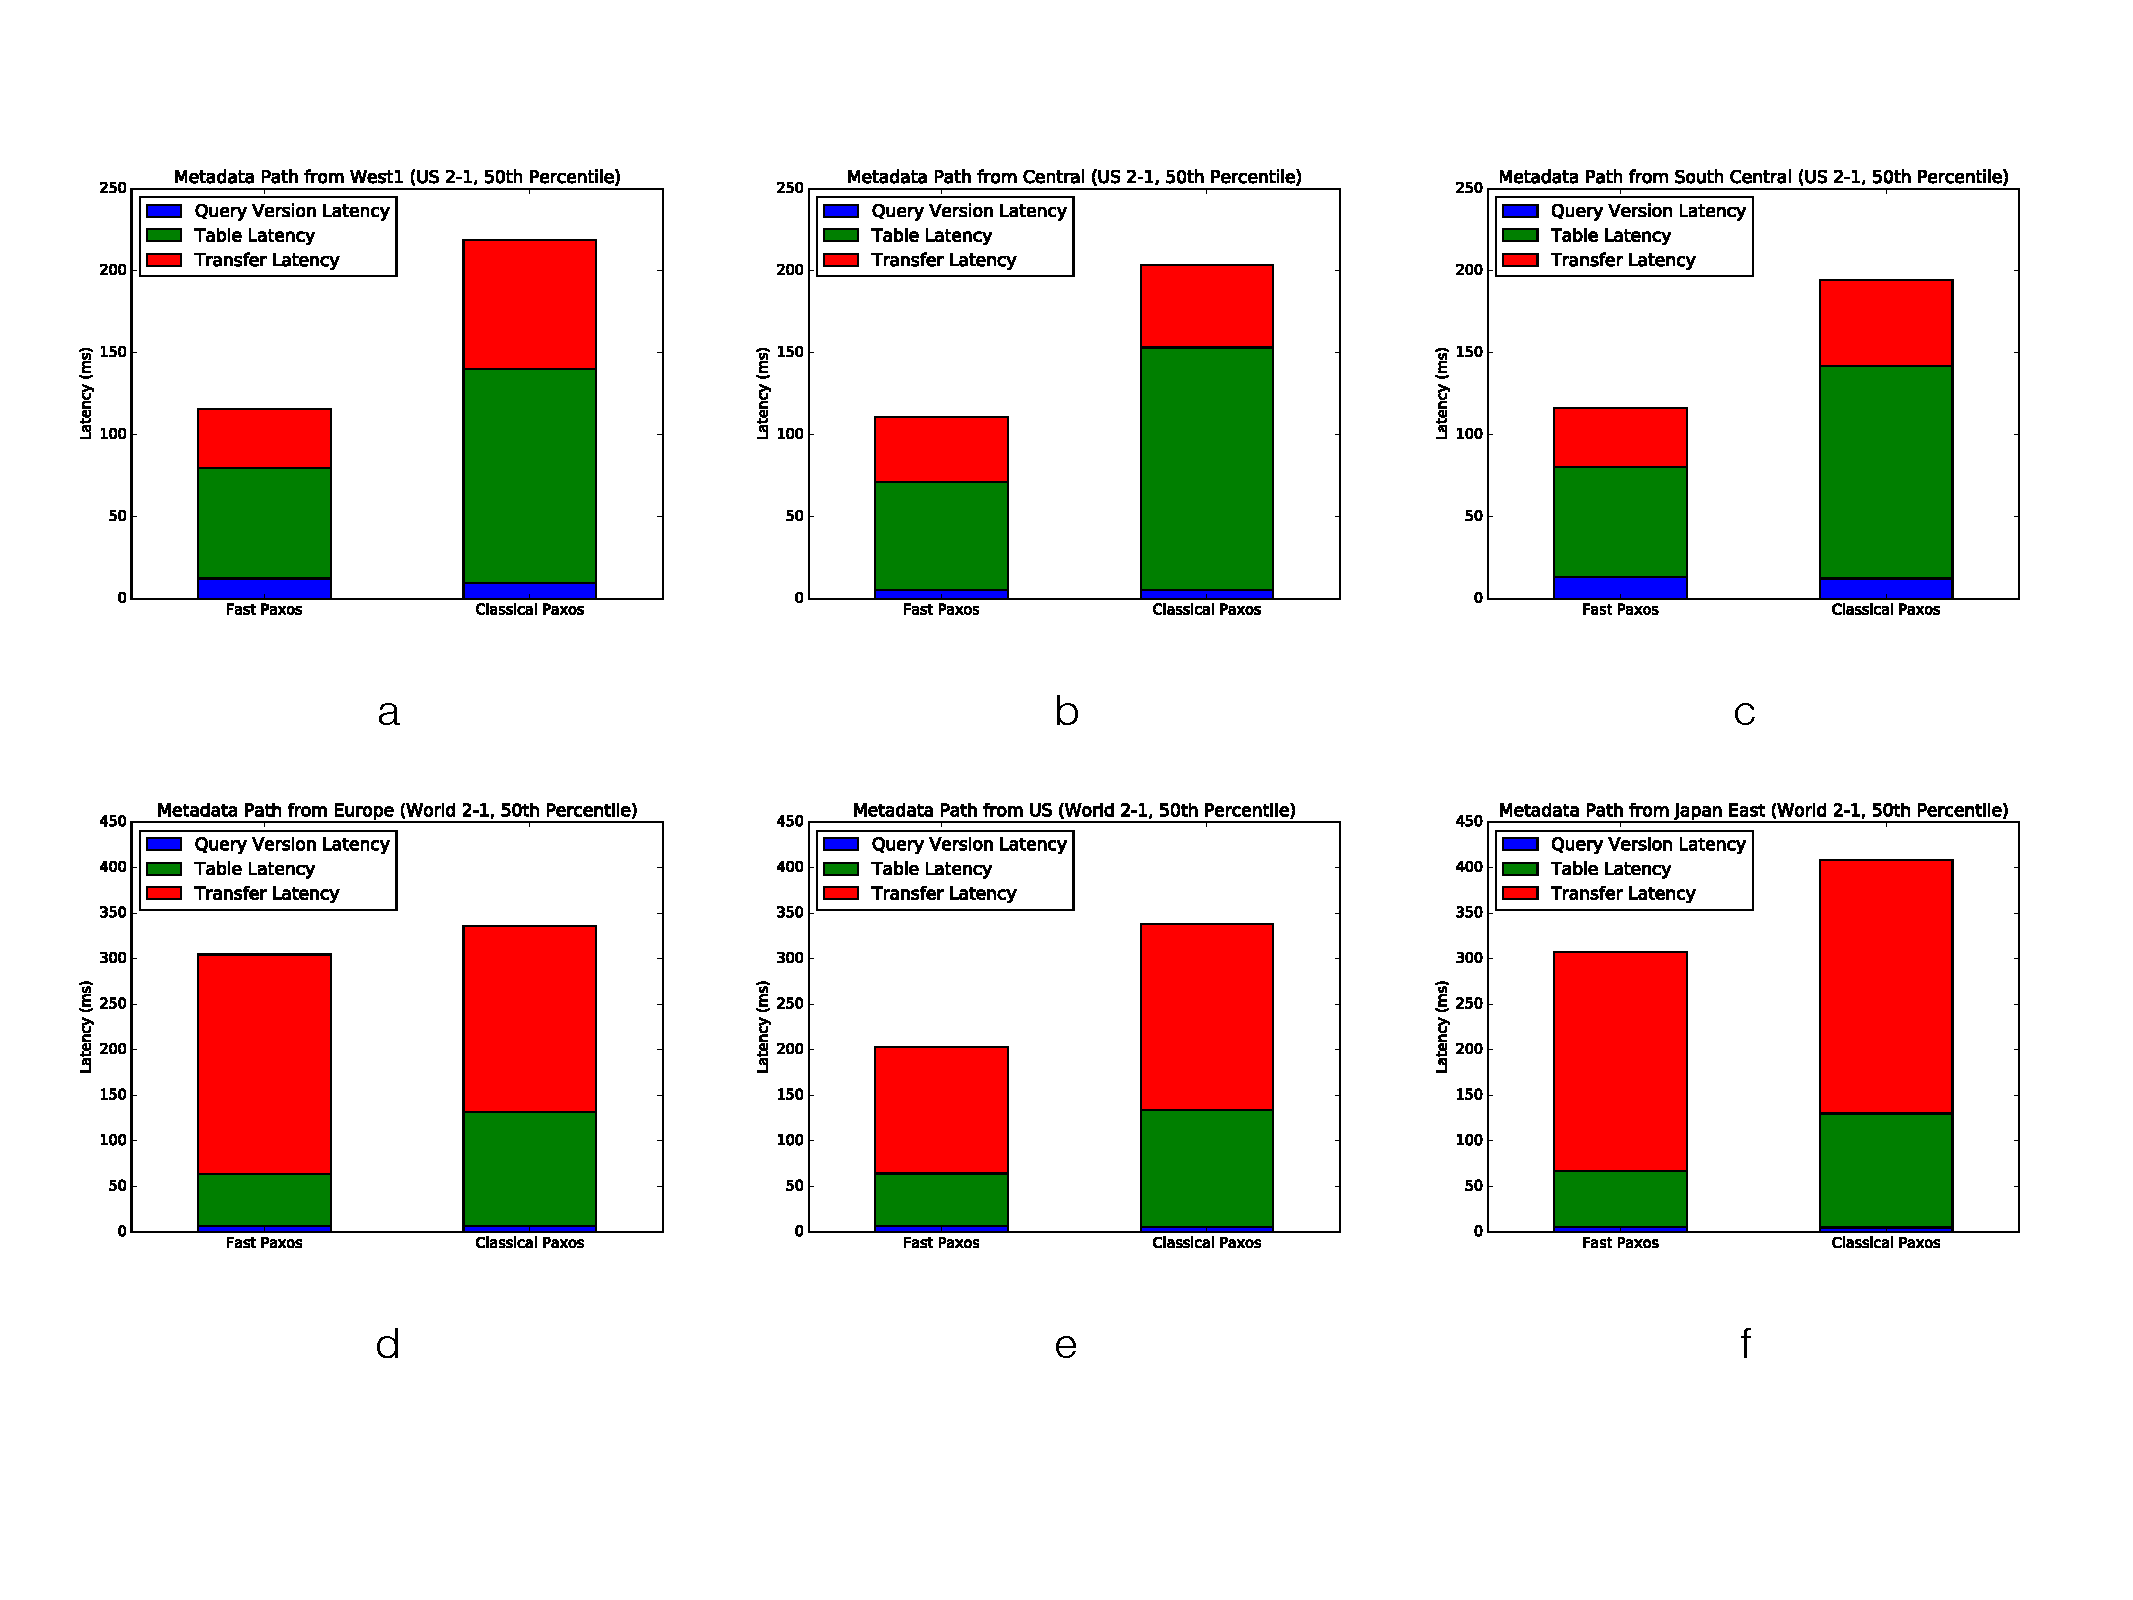
\includegraphics[width=\linewidth]{images/Metadata_vs}
      \caption{Fast Paxos and Classic Paxos Comparison}
      \label{fig:metadata}
%  }
\end{figure}

\subsection{\name Latency}
The design of Giza went through multiple iterations and this section illustrates the performance gain in latency for each iteration. Through our workload analysis, we chose to erasure code objects with size larger 4MB. Hence, we focus on the {\em put} and {\em get} latency of 4MB objects in the evaluation. For the interest of space, we chose the 2-1-World configuration where US Central generates all requests as representative of the performance gain seen in other configurations.

\subsubsection{Giza Put Latency}
%\subsubsection{Giza Latency}

%\begin{figure}[t]
%  \centerline {
%    \begin{subfigure}{0.20\textwidth}
%      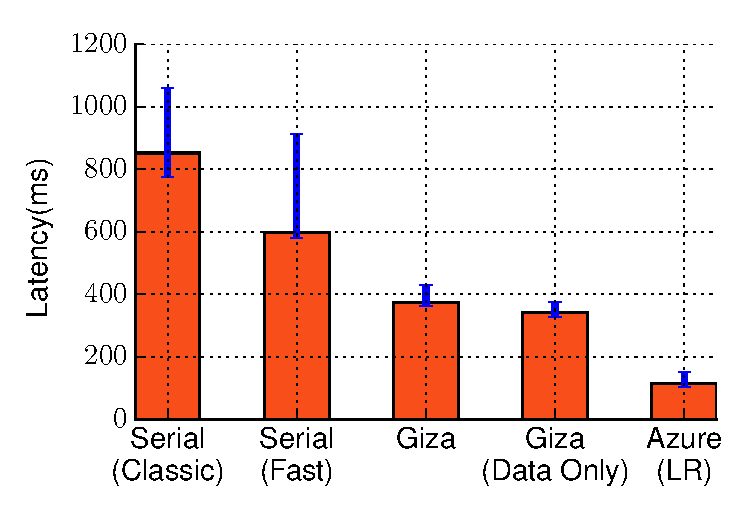
\includegraphics[width=\linewidth]{plots/giza_lat_put}
%      \caption{Put}
%      \label{fig:eval_giza_put}
%    \end{subfigure}
%    \begin{subfigure}{0.20\textwidth}
%      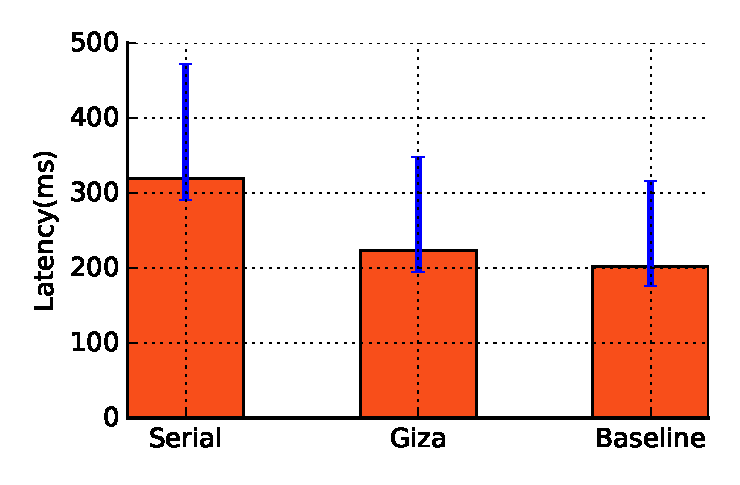
\includegraphics[width=\linewidth]{plots/giza_lat_get}
%      \caption{Get}
%      \label{fig:eval_giza_get}
%    \end{subfigure}
%  }
%  \caption{\name Overall Latency}
%  \label{fig:geo_tpcc}
%\end{figure}

%%% Local Variables:
%%% mode: latex
%%% TeX-master: "main"
%%% End:


Figure~\ref{fig:eval_giza_put} shows the \name overall {\em put} latency for 4MB data. We compare Giza with two previous iterations where the metadata path is not parallelized with the data path. In the first iteration, Giza runs the data path first. Upon success, Giza runs the metadata path with Classic Paxos implementation. In the second iteration, we replaced Classic Paxos with Fast Paxos and see the performance gain described previously. While parallelizing metadata path with data path can results in extra metadata or data clean up if one of them fails, the performance gain is significant. We also included a baseline which is the blob store latency from the requester (US Central) to the furthest data center (Japan East). Finally, we include the latency for storing the 4MB data directly to Azure storage, which is locally replicated.

The results show that \name's performance beats the other two alternatives in the common case and has closest
latency to the baseline. The median latency of \name put is 374 ms, which is only 30 ms
higher than the baseline. This is due to the latency of erasure coding 4mb data. On the other hand, the serial classic paxos version takes 
852 ms, and the serial fast paxos version takes 598 ms. Compared to local replication, the latency cost of tolerating data center failure with Giza is a little more than 3 times.

\subsubsection{Giza Get Latency}

Similar to the put test, we did a \name get test, as shown in Figure~\ref{fig:eval_giza_get}. The alternative design here is the non-optimistic {\em get } where the most current version for a blob is not assumed to be stored in the current data center. Hence, the metadata path and data path are executed sequentially. We see the performance gain from the pessimistic version with a median latency 419 ms to the optimistic version's 223 ms. Giza's get latency is higher than the baseline by 190 ms. The gap between \name and baseline is higher because in the get operation \name needs to do a local table retrieve first before starting the datapath. Here the latency cost of erasure encoding on the read path with Giza is roughly twice that of reading from a locally redundant Azure storage.

%The results are expected. The \name put latency consists of a 
%metadata put latency and datapath latency. 



\comment{

% \begin{figure}[!h]
% \centering
%   \subfloat[Giza Put 99th Percentile]{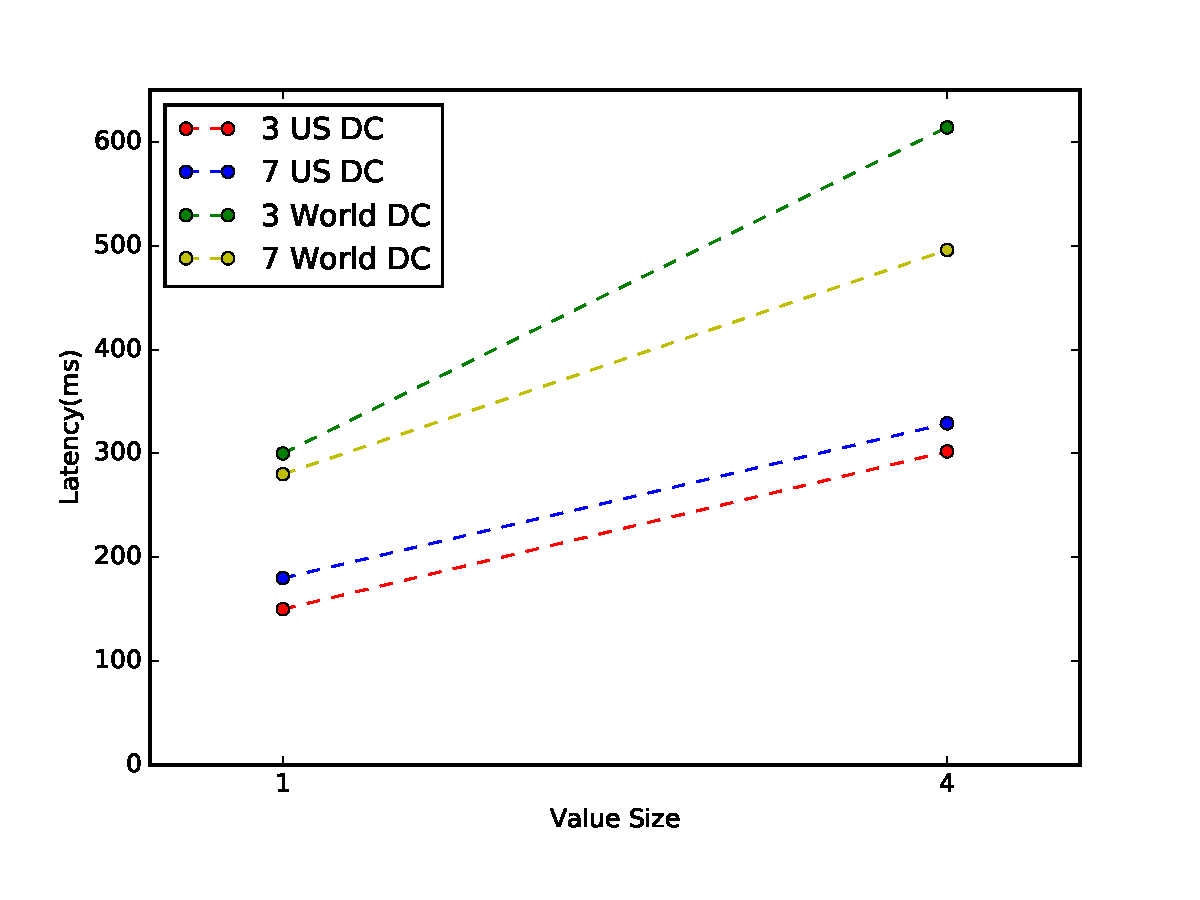
\includegraphics[width=0.5\textwidth]{images/write_latency}\label{fig:f1}}
%   \subfloat[Giza Get 99th Percentile]{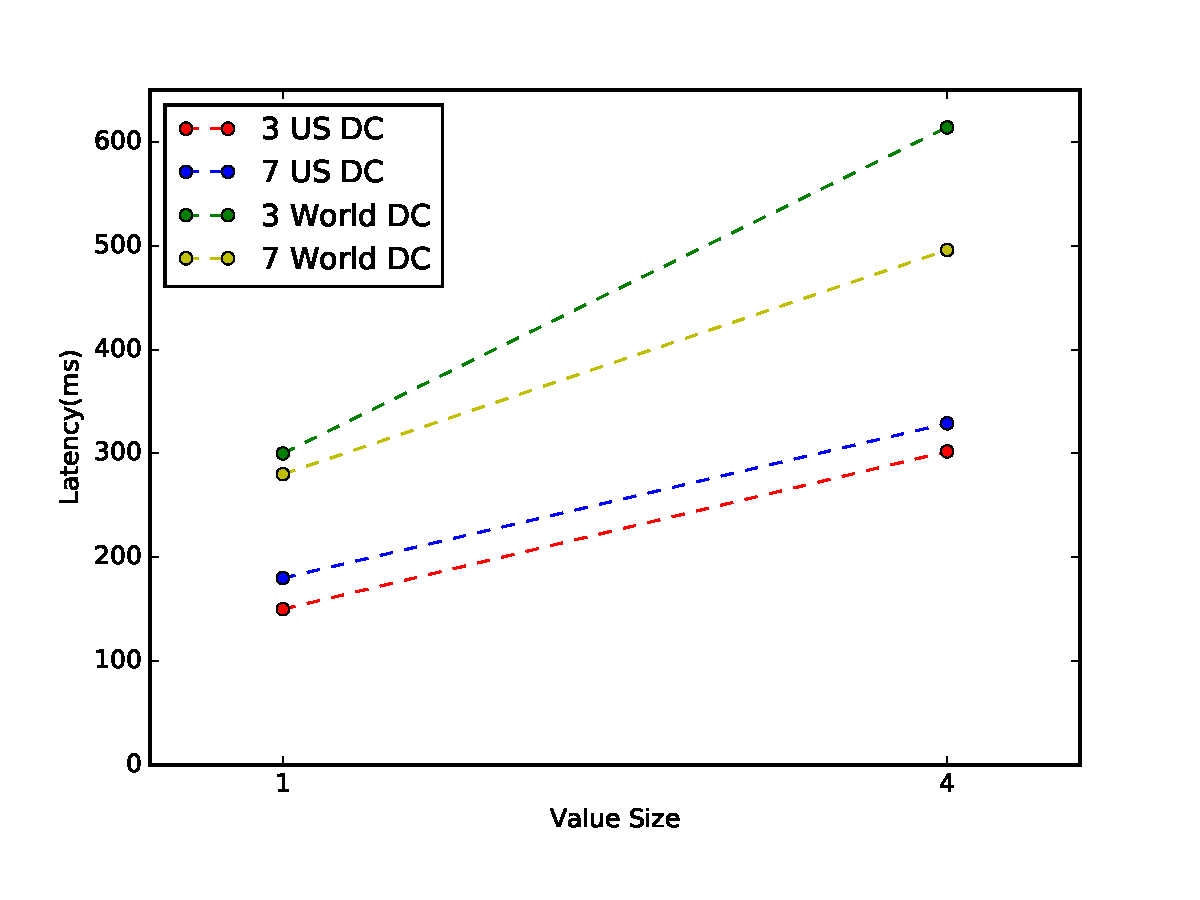
\includegraphics[width=0.5\textwidth]{images/write_latency}\label{fig:f2}}
% \caption{Comparison of latency of the four configurations}
% \end{figure}
\subsection {Different Configurations}
\sm {
  In this section, I will provide a latency graph (put and get) of all the 4 different configurations. The x axis is the size of the objects and the y axis is the latency. This section is to illustrate the trade off between storage efficiency and read latency. 
}

}

\subsection{Footprint Impact}


\begin{figure}[t]
%  \centerline {
    \begin{subfigure}{0.40\textwidth}
      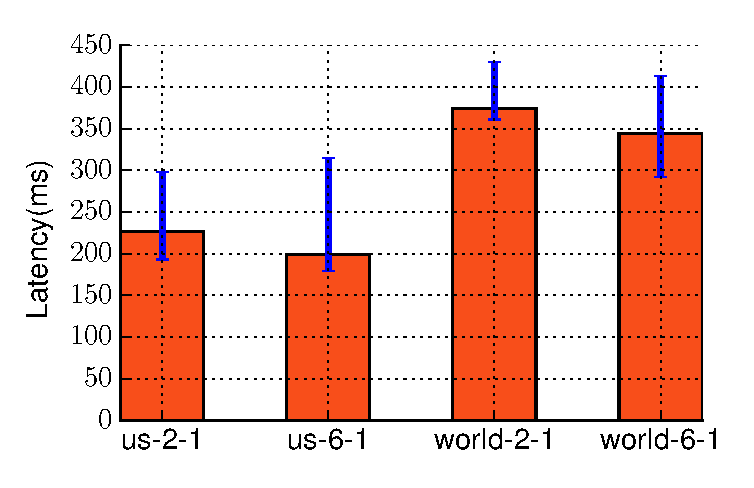
\includegraphics[width=\linewidth]{plots/giza_four_put}

      % \placeholder{
      %   x-axis: \# clients / partition\\
      %   y-axis: cluster throughput\\
      %   lines: \name{}, OCC, 2PL, TAPIR\\
      %   }
%                \vspace{-1\baselineskip}
      \caption{Put}
      \label{fig:eval_giza_put_four}
    \end{subfigure}
%    \begin{subfigure}{0.33\textwidth}
%      \includegraphics[width=\linewidth]{figs/graphs/multi_dc/tpcc/tpcc_NEW_ORDER_tpcc_client_lat90.eps}
%
%      % \placeholder{
%      %   x-axis: \# clients / partition\\
%      %   y-axis: latency (median, p90, p99)\\
%      %   (maybe only show median and p99 or just median and report typical distribution)\\
%      %   lines: \name{}, OCC, 2PL, TAPIR\\
%      % }
%      \caption{90\% Latency}
%      \label{fig:geo_tpcc_latency}
%    \end{subfigure}
    \begin{subfigure}{0.40\textwidth}
      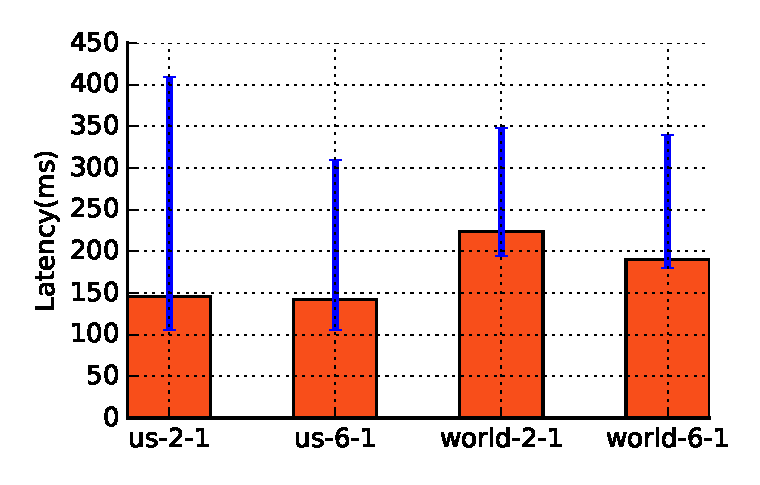
\includegraphics[width=\linewidth]{plots/giza_four_get}

      % \placeholder{
      %   x-axis: \# clients / partition\\
      %   y-axis: commit rate\\
      %   lines: \name{}, OCC, 2PL, TAPIR\\
      % }
      %\includegraphics[width=\linewidth]{fig/kodiak/tpcc_mix_10_nlog_ct_cr.pdf}
%                \vspace{-1\baselineskip}
      \caption{Get}
      \label{fig:eval_giza_get_four}
    \end{subfigure}
%  }
  \caption{Performance for \name in different setups}
\end{figure}

%%% Local Variables:
%%% mode: latex
%%% TeX-master: "main"
%%% End:


\name offers customers the flexibility to choose the set of data centers, as well as the erasure coding schemes. As the main goal of Giza is storage cost reduction, we want to encourage erasure encoding with more numbers of data fragments. Because Giza’s latency performance is determined by the max of the data path and the metadata path and data path is most often the dominant latency, erasure coding with higher number of data fragments can actually improve latency performance. This is because more data fragments means that less bytes are sent to each storage, reducing the overall data path latency. Figure~\ref{fig:eval_giza_put_four} and  Figure~\ref{fig:eval_giza_get_four} illustrate this in our four configurations with 4MB data, with all requests generated from US-Central. This improvement of performance with higher configurations occurs when the max distance between the data centers in the higher configuration group (7 data centers) is not more than the max distance between the data centers in the lower configuration group (3 data centers).


\subsection{Comparing Giza with CockroachDB}
We only compare Giza's US-2-1 configuration with CockroachDB since CockroachDB currently does not fully support world wide geo-replication. We also don't include comparison to  the US-6-1 scheme in the interest of space.

We implemented Giza put and get as transactions. Because CockroachDB fully supports ACID transactions, we can use CockroachDB to build a strongly consistent key value store that encodes objects across multiple data centers. To do this, we create four different tables: a metadata table and 3 tables that serves as key-value stores for each of the data centers. The metadata table is replicated across all three data centers, once in each data center, and can tolerate one data center failure. Each of the remaining tables is replicated 3 times in its respective data center. Since CockroachDB uses Paxos for replication, the write critical path only requires the completion of 2 our of 3 replications. This is to match the local replication factor in the Azure storage where each blob is synchronously replicated once on the write critical path.

The implementation of Giza put as a transaction consists of storing each data fragments at the corresponding key-value table and storing the metadata information in the metadata table. This transaction involves all four tables for a 2,1 configuration. Figure~\ref{fig:eval_cock_put} compares the latency performance of the two. Here Giza outperforms CockroachDB significantly.
However CockroachDB is currently not suited for storing large objects, as specified by the developers. We also tested CockroachDB with 128KB objects (This is 64KB after encoding, which is the largest size CockroachDB can handle before performance degradation). However, even with just 128KB (blue bar), the performance of CockroachDB is still worse than the performance of Giza even with 4MB objects.

The implmentation of Giza get as a transaction consists of reading from the metadata table and reading the minimum amount of data fragments, in this case two, from the key value tables. This transaction involves three out of the four tables. Figure~\ref{fig:eval_cock_get} shows the performance comparison. Here CockroachDB performs better than Giza. However, this is not surprising. CockroachDB reads directly from HDD, which is faster than Giza's read from the Azure storage. However, when we replace Giza's storage layer with hdd, Giza outperforms CockroachDB.

\begin{figure}[t]
%  \centerline {
    \begin{subfigure}{0.45\textwidth}
      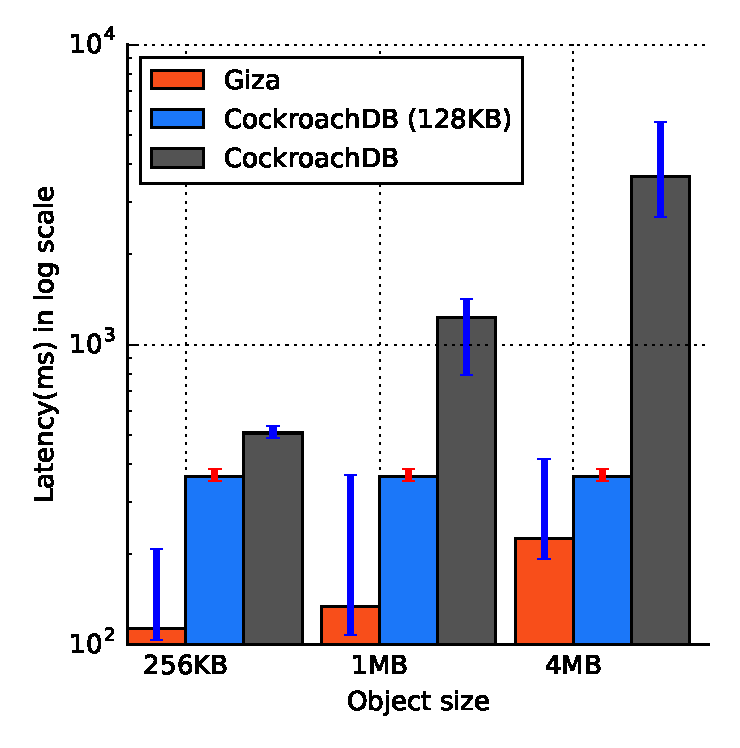
\includegraphics[width=\linewidth]{plots/giza_cock_put}

      % \placeholder{
      %   x-axis: \# clients / partition\\
      %   y-axis: cluster throughput\\
      %   lines: \name{}, OCC, 2PL, TAPIR\\
      %   }
%                \vspace{-1\baselineskip}
      \caption{Put}
      \label{fig:eval_cock_put}
    \end{subfigure}
%    \begin{subfigure}{0.33\textwidth}
%      \includegraphics[width=\linewidth]{figs/graphs/multi_dc/tpcc/tpcc_NEW_ORDER_tpcc_client_lat90.eps}
%
%      % \placeholder{
%      %   x-axis: \# clients / partition\\
%      %   y-axis: latency (median, p90, p99)\\
%      %   (maybe only show median and p99 or just median and report typical distribution)\\
%      %   lines: \name{}, OCC, 2PL, TAPIR\\
%      % }
%      \caption{90\% Latency}
%      \label{fig:geo_tpcc_latency}
%    \end{subfigure}
    \begin{subfigure}{0.45\textwidth}
      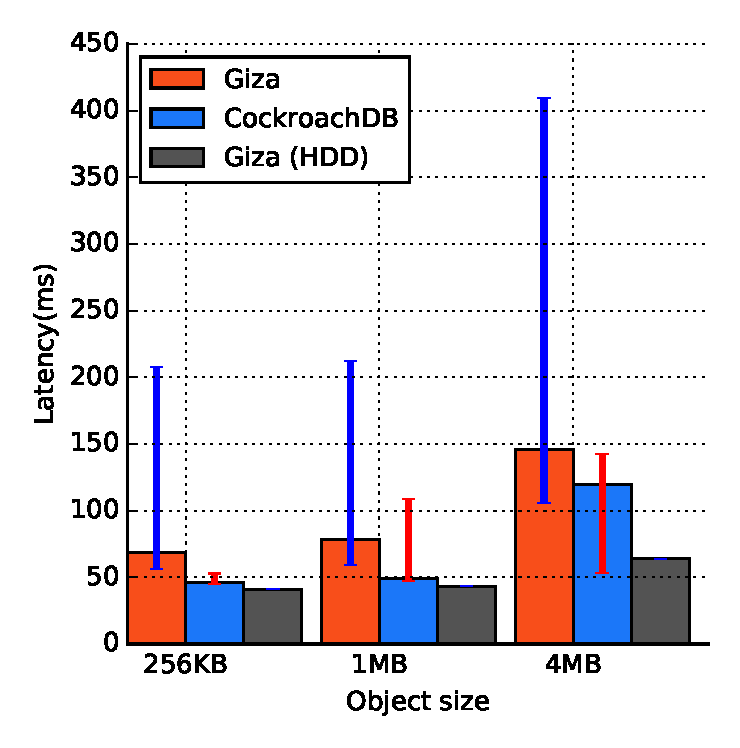
\includegraphics[width=\linewidth]{plots/giza_cock_get}

      % \placeholder{
      %   x-axis: \# clients / partition\\
      %   y-axis: commit rate\\
      %   lines: \name{}, OCC, 2PL, TAPIR\\
      % }
      %\includegraphics[width=\linewidth]{fig/kodiak/tpcc_mix_10_nlog_ct_cr.pdf}
%                \vspace{-1\baselineskip}
      \caption{Get}
      \label{fig:eval_cock_get}
    \end{subfigure}
%  }
  \caption{Performance for \name in different setups}
\end{figure}
% \begin{figure}[t]
% %  \centerline {
%       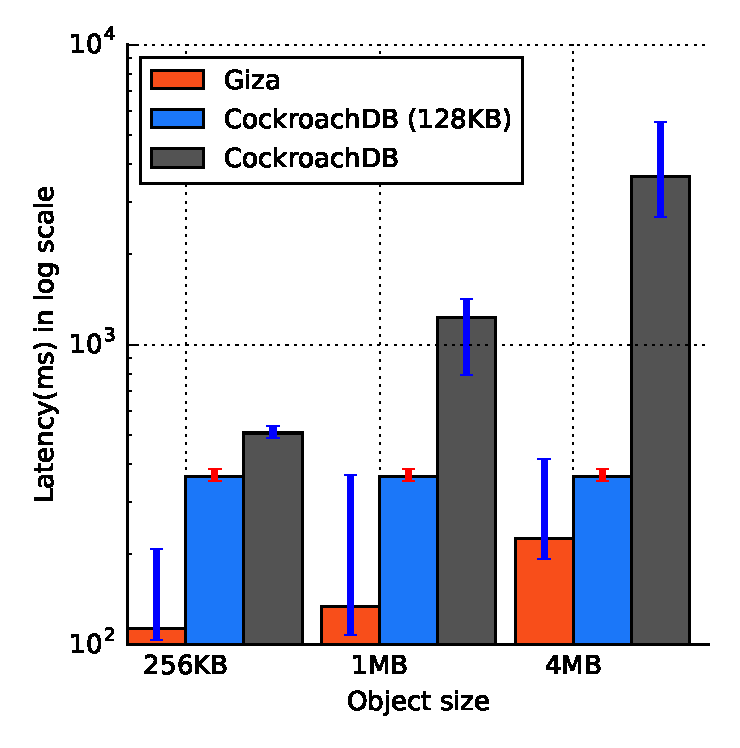
\includegraphics[width=\linewidth]{plots/giza_cock_put}
%       \caption{CockroachDB vs Giza Put with various object sizes}
%       \label{fig:eval_cock_put}
% %  }
% \end{figure}

% %\begin{figure}[t]
% %  \centerline {
% %      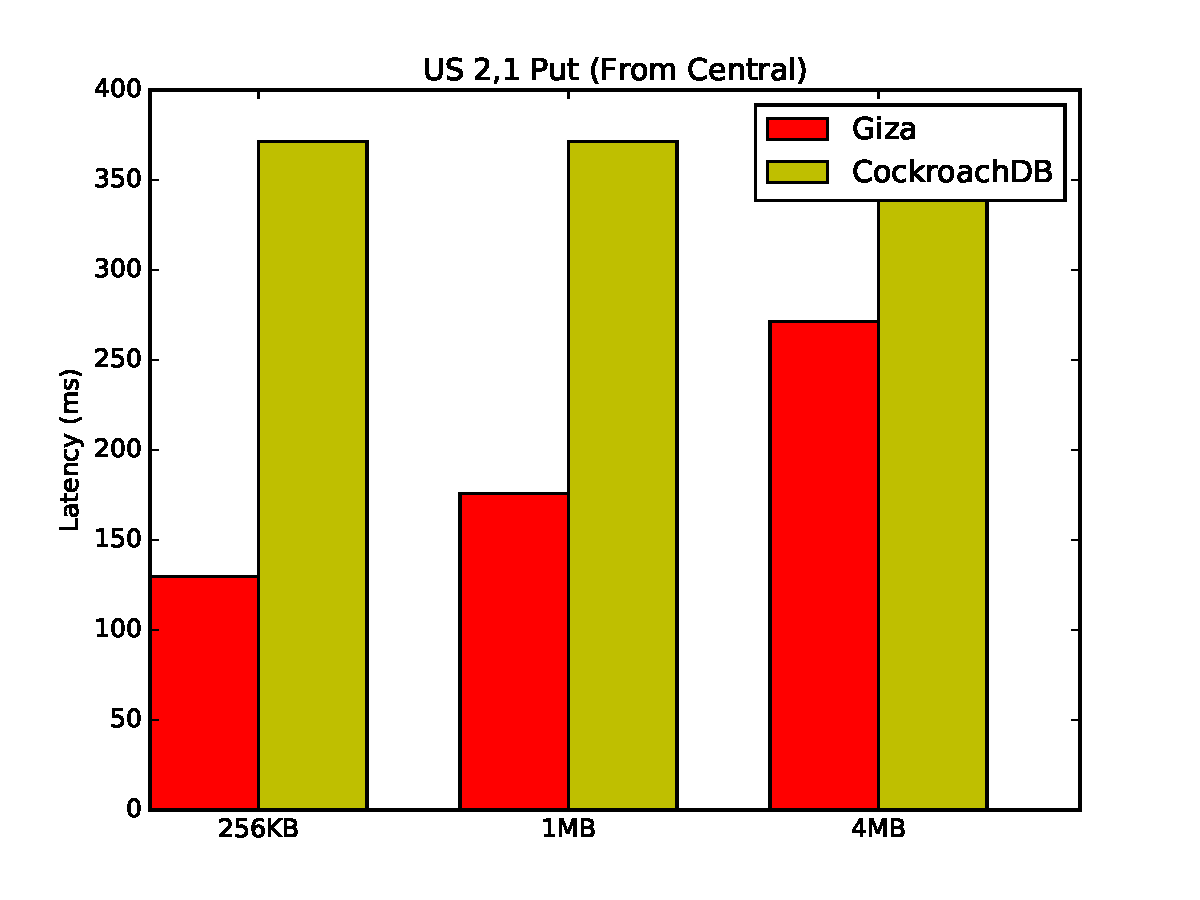
\includegraphics[width=\linewidth]{images/cockroach_vs_giza_put_128}
% %      \caption{CockroachDB vs Giza with various object sizes}
% %      \label{fig:eval_cock_put2}
% %  }
% %\end{figure}

% \begin{figure}[t]
% %  \centerline {
%       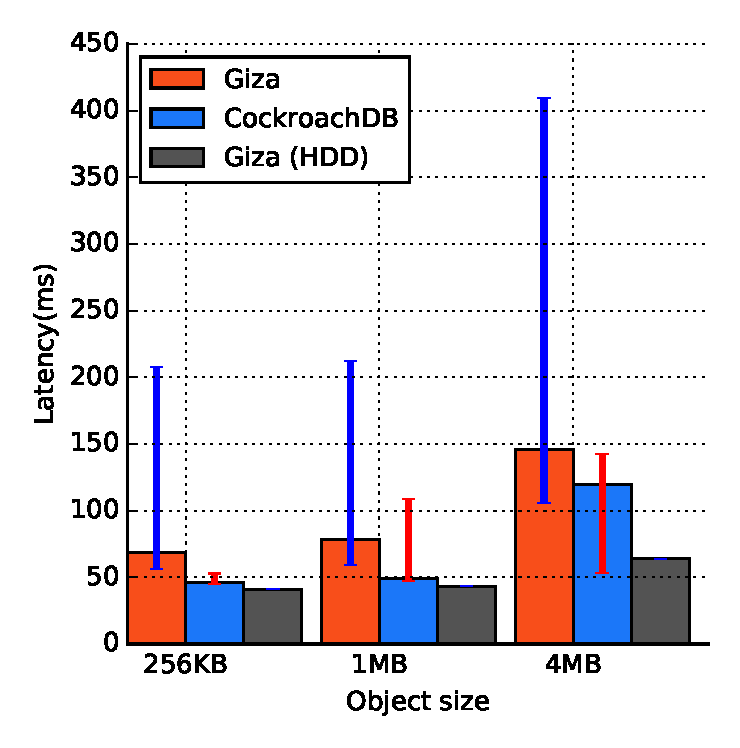
\includegraphics[width=\linewidth]{plots/giza_cock_get}
%       \caption{CockroachDB vs Giza Get with various object sizes}
%       \label{fig:eval_cock_get}
% %  }
% \end{figure}
%%% Local Variables:
%%% mode: latex
%%% TeX-master: "main"
%%% End:


\subsection{Giza Contention}

We evaluate the latency performance of Giza’s metadata path under contention with the 2-1-US configuration. Figure~\ref{fig:gizacontentionbar} compares the performance of no contention workload vs full contention workload. In both set up, all requests are generated from the same data center (US-Central). In the case of contention, two Giza nodes within the data center issue concurrent put to the same key. During contention, at least one of the fast paxos round will fail. The Giza node that failed the paxos round will then run a classic paxos round. We implement a exponential back off strategy starting with the median latency of a single RTT whenever prepare phase or accept phase fails in the classic round. 

In most cases, both the fast rounds fail. In this scenario, one of the the Giza node will fail either at the prepare phase or the accept phase. In the former case, the expected latency is 6 RTT: Fast round -> Prepare Phase -> Back off -> Prepare Phase -> Accept Phase -> Fast Round.In the latter case, the expected latency is 7 RTT: Fast Round -> Prepare Phase -> Accept Phase -> Back off -> Prepare Phase -> Accept Phase -> Fast Round. This is consistent with the median contention latency.

It is important to note that while Giza is correct under contention, it is not optimized for contention. This is because Giza is designed to handle real life workload with little to no contentions. From Section~\ref{sec:motivation}, we observe that only 0.5\% of Giza's updates are concurrent (within 1 seconds). Figure~\ref{fig:gizacontentioncdf}  compares the estimated latency cdf of Giza under a no-contention workload with workload driven by Section~\ref{sec:motivation}. 

%We evaluate the latency performance of Giza’s metadata path under contention with our 2-1-US configuration. From our One Drive analysis, only 0.5\% of all updates happen concurrently. To simulate this workload, we run 1000 metadata put where 0.5\% of puts are concurrent puts from two Giza nodes. All requests are from the same data center (US Central). Figure~\ref{fig:gizacontentioncdf} shows the cdf of running Giza with One Drive’s workload distribution when compared with workload with no contentions. Since only a small number of puts are concurrent, the cdf of the contention workload follows the same curve as that of the no contention workload until 95\%. 

%During contention, there may be multiple interleaving of our metadata path protocol. In the best scenario, on one metadata path, the fast paxos round succeeds. The ideal scenario here is for the Giza node which failed the fast round to wait until the version number is updated. It will then run a new fast round for the new version. However it is possible for both fast found to fail. In this scenario, the version number never increases. In this case, the Giza nodes will have to run classical paxos. We use the same random back off used in other paxos system, taking into account the median latency for each Paxos phase. Figure~\ref{fig:gizacontentionbar}  illustrates the contention latency when compared to the no contention latency.

\begin{figure}[t]
%  \centerline {
      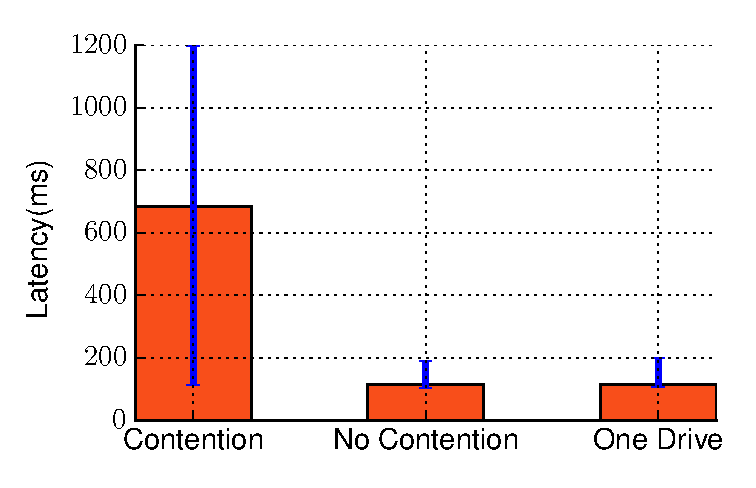
\includegraphics[width=0.40\textwidth]{plots/contention_bar}
      \caption{Contention vs No Contention}
      \label{fig:gizacontentionbar}
%  }
\end{figure}


%We evaluate the throughput of Giza in a local-area cluster. Figure xxx shows the result of a single Giza deployment for storing 4MB objects. The 24 ops per second equates to 144MB per second which is consistent with the 150MB per second cap for each Azure Virtual Machine. For each additional Giza node, we add three storage accounts. This is to deal with the current throughput cap per storage account, which is 200MB per second.  The keyspace is partitioned equally among sets of three storage accounts. Figure~\ref{fig:gizathroughput} depicts the throughput as we increase Giza nodes. Here, the throughput increases linearly. 

%\begin{figure*}
%\begin{tabular}{c|c|c|c|c|c}
%Giza Nodes & 1 & 2 & 3 & 4 & 5\\
%\hline
%ops/second & 24 & 34 & 49 & 73 & 96 \\
%MB/second & 144 & 204 & 294 & 438 & 576\\ 
%\end{tabular}
%\caption{Throughput result of local Giza cluster\label{fig:gizathroughput}} 
%\end{figure*}

%To set up CockroachDB, we use the same Azure virtual machine instances and run a single CockroachDB node. We followed the recommended production settings by the developers of CockroachDB when deploying these instances. For example, on the same virtual machine, we also run NTP to provide moderately accurate time to preserve data consistency. Other optimizations can be found on the CockroachDB website. We only benchmark CockraochDB against Giza in the 3 dc cluster scenario since we want the fault tolerance level to be the same for the comparisons.
%Since variability in latency is a factor when benchmarking cloud storage, we run all our experiments at approximately the same time.
%Since latency is an issue, we run all our experiments at around the same time.
%We experimented with different erasure coding schemes
% For all experiments, we deployed a single virtual machine (16 cores, 56 GB of RAM, 800 GB SSD, and gigabit ethernet) for each geographical region. We use the same virtual machines for setting up the Cassandra and CockroachDB clusters. The client issuing the requests runs on one of the virtual machine that is also part of the cluster. 
% To set up Giza, we also had to deployed both a table service and a blob service provided by the cloud service platform. The granularity of replication for these services varies from provider to provider but we always choose the replication level to match that of the regional replication. This means that as long as there’s no dc outage, the data would not be lost. For each data center, we run a Giza node frontend with the virtual machine. The Giza node can service requests from a client running in the virtual machine. In addition, requests to its local table and blob storage from other Giza nodes also go through the Giza node frontend in the form of an RPC call. This is to avoid unecessary WAN round trips when dealing with complicated table and blob storage operations. 
%\begin{figure}[t]
%  \centerline {
    \begin{subfigure}{0.45\textwidth}
      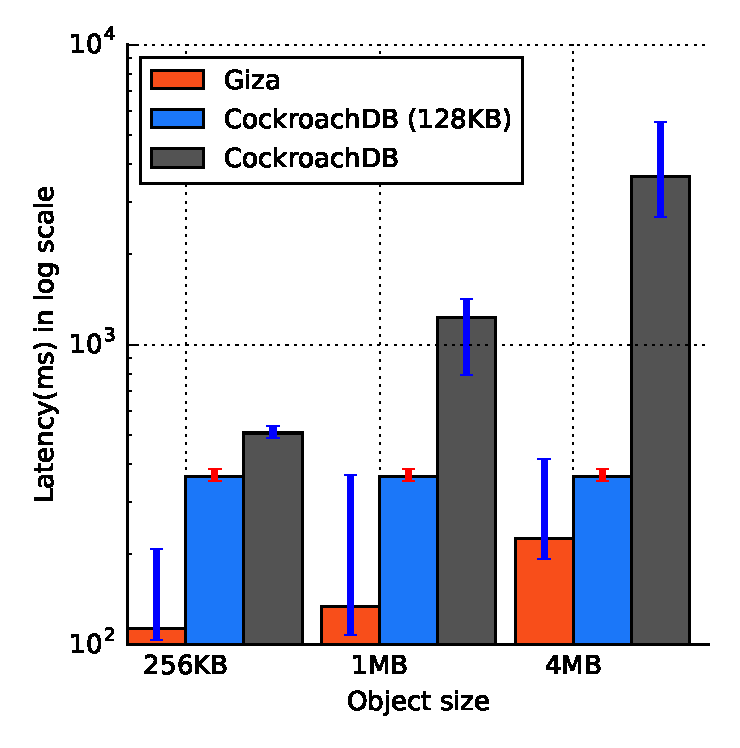
\includegraphics[width=\linewidth]{plots/giza_cock_put}

      % \placeholder{
      %   x-axis: \# clients / partition\\
      %   y-axis: cluster throughput\\
      %   lines: \name{}, OCC, 2PL, TAPIR\\
      %   }
%                \vspace{-1\baselineskip}
      \caption{Put}
      \label{fig:eval_cock_put}
    \end{subfigure}
%    \begin{subfigure}{0.33\textwidth}
%      \includegraphics[width=\linewidth]{figs/graphs/multi_dc/tpcc/tpcc_NEW_ORDER_tpcc_client_lat90.eps}
%
%      % \placeholder{
%      %   x-axis: \# clients / partition\\
%      %   y-axis: latency (median, p90, p99)\\
%      %   (maybe only show median and p99 or just median and report typical distribution)\\
%      %   lines: \name{}, OCC, 2PL, TAPIR\\
%      % }
%      \caption{90\% Latency}
%      \label{fig:geo_tpcc_latency}
%    \end{subfigure}
    \begin{subfigure}{0.45\textwidth}
      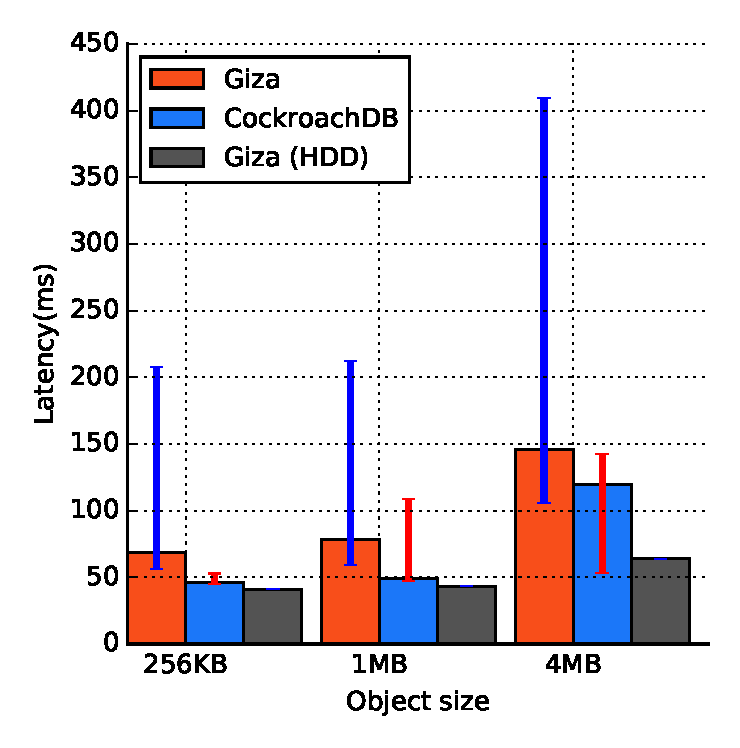
\includegraphics[width=\linewidth]{plots/giza_cock_get}

      % \placeholder{
      %   x-axis: \# clients / partition\\
      %   y-axis: commit rate\\
      %   lines: \name{}, OCC, 2PL, TAPIR\\
      % }
      %\includegraphics[width=\linewidth]{fig/kodiak/tpcc_mix_10_nlog_ct_cr.pdf}
%                \vspace{-1\baselineskip}
      \caption{Get}
      \label{fig:eval_cock_get}
    \end{subfigure}
%  }
  \caption{Performance for \name in different setups}
\end{figure}
% \begin{figure}[t]
% %  \centerline {
%       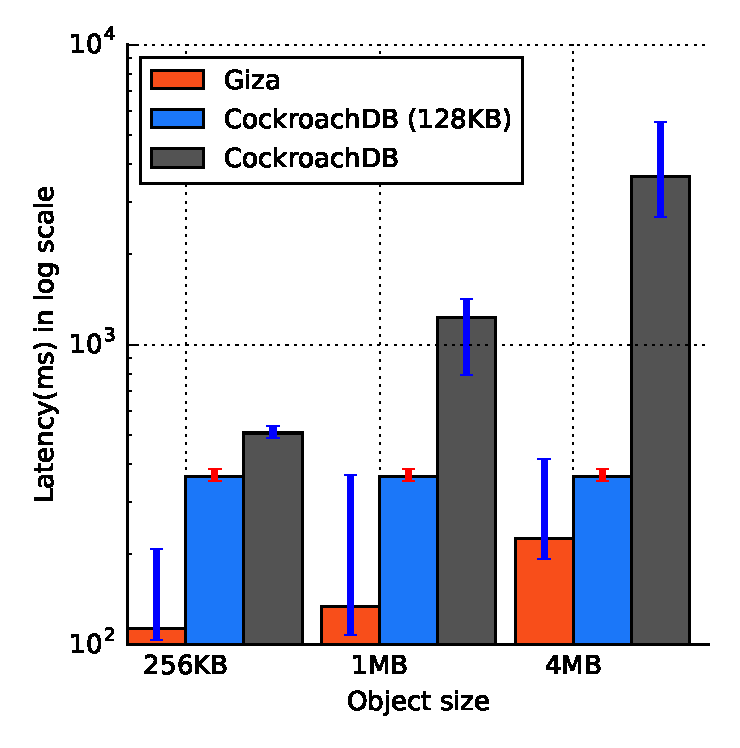
\includegraphics[width=\linewidth]{plots/giza_cock_put}
%       \caption{CockroachDB vs Giza Put with various object sizes}
%       \label{fig:eval_cock_put}
% %  }
% \end{figure}

% %\begin{figure}[t]
% %  \centerline {
% %      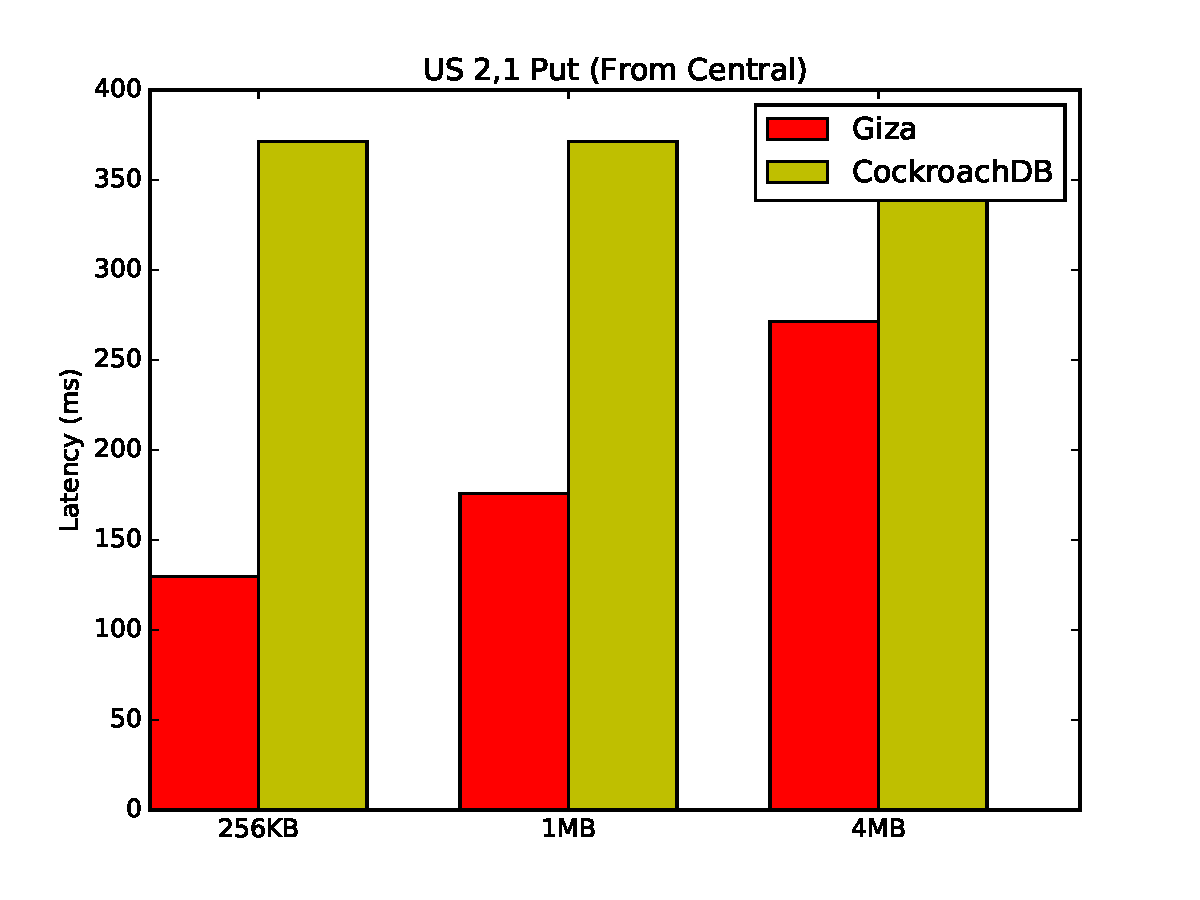
\includegraphics[width=\linewidth]{images/cockroach_vs_giza_put_128}
% %      \caption{CockroachDB vs Giza with various object sizes}
% %      \label{fig:eval_cock_put2}
% %  }
% %\end{figure}

% \begin{figure}[t]
% %  \centerline {
%       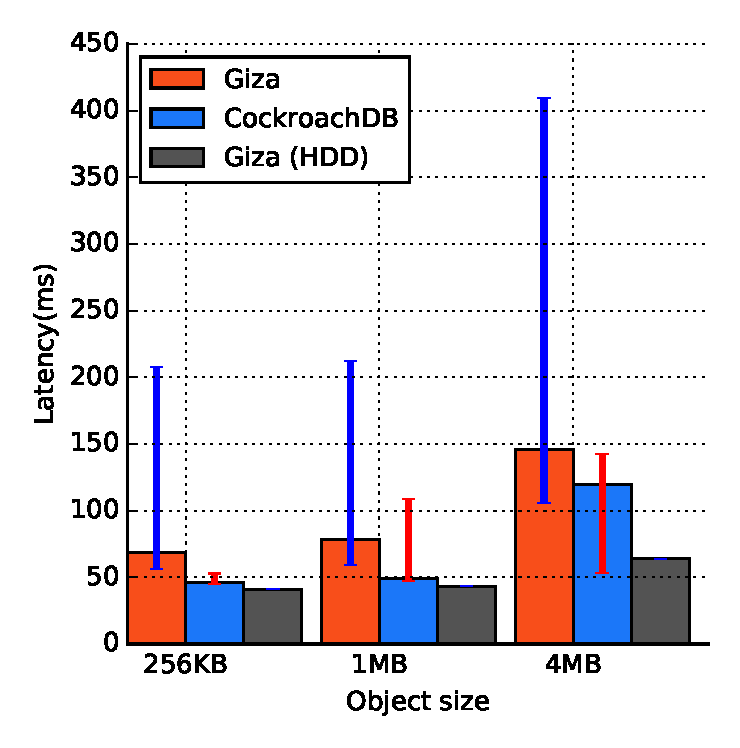
\includegraphics[width=\linewidth]{plots/giza_cock_get}
%       \caption{CockroachDB vs Giza Get with various object sizes}
%       \label{fig:eval_cock_get}
% %  }
% \end{figure}
%%% Local Variables:
%%% mode: latex
%%% TeX-master: "main"
%%% End:


%\sm {
%  In this section, I will have two graphs. One comparing Giza's full write path with CockroachDB's full replication. Another one is comparing the metadata path with cockroach db. This is to show, hopefully, that the fast paxos scheme is better. I will probably have 3 graphs each making request from one of the three datacenters. Due to multipaxos, there might be extra latency for cockroachdb's case.
%}
%We benchmark the performance of Giza with CockroachDB in two cases. In the first case, we use CockroachDB as a geo-replicating blah blah blah. Here is the result.
%In the second case, we used cockroachdb's transaction to simulate what we are doing with Giza. Blah blah blah, here is the result.
%64K $\sim$ 16MB

%X-axis: Value size
%Y-axis: 50\% Read latency

%X-axis: Value size
%Y-axis: 90\% Read latency

%X-axis: Value size
%Y-axis: 99\% Read latency

%Same for write

%[adding cpu results in a table]

% \subsection{Large object}
% 256MB $\sim$ 1GB

% X-axis: Value size
% Y-axis: Average Read latency

% X-axis: Value size
% Y-axis: Average Write latency


% \subsection{Contention}

% Fixed object size
% X-axis: zipf coefficient
% Y-axis: 50\%, 90\%, 99\% Read/Write Latency


% \subsection{Real workload}
% Table.


%%% Local Variables:
%%% mode: latex
%%% TeX-master: "main"
%%% End:

